
\chapter{Reduction}







\section{Introducing Reduction}


We want to formalise our intuition that certain problems are \textit{computationally harder} than
others. We also want to formalise the idea that some problems have the 
same difficulty or are \textit{computationally equivalent}. 
These two ideas are formalised using the notion of \textit{language reduction}.

Given two languages: $L_1 \subseteq \Sigma^{*}_1$
and $L_2 \subseteq \Sigma^{*}_2$, a \textit{$C$-time reduction of $L_1$ to $L_2$}
is defined to be computable function $r : \Sigma^{*}_1 \rightarrow \Sigma^{*}_2$
such that:

\begin{itemize}   
\renewcommand{\labelitemi}{$\Box$}
\item \textbf{Codomain is a subset} The codomain of $f$ is a subset of  $L_2$. 
In other words if instance $x$ is in $L_1$ then there is some instance $r(x)$ in $L_2$. 
And if $f(x)$ is an instance in $L_2$, we will there will be an instance x in $L_1$. 
\item \textbf{Computable in $C$-time} The function $f$ can be computed 
by our computational model, where $C$ 
is some language complexity class. 
\end{itemize} 

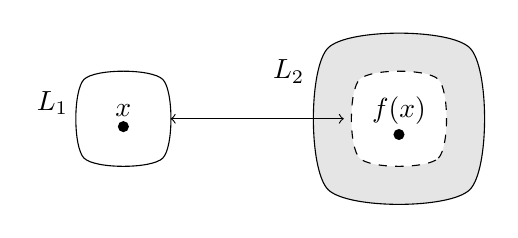
\begin{tikzpicture}
% left
\node (x) at (-0.4,0.7) {$L_1$};
\draw plot [smooth cycle] coordinates {(0,0) (1,0) (1,1) (0,1) };
\node (x) at (0.5,0.6) {$x$};
\fill (x.south) circle [radius=2pt];
% right
\node (x) at (2.6,1.1) {$L_2$};
\draw[fill=black!10] plot [smooth cycle] coordinates {(3.1,-0.4) (4.9,-0.4) (4.9,1.4) (3.1,1.4) };
\draw[dashed, fill=white] plot [smooth cycle] coordinates {(3.5,0) (4.5,0) (4.5,1) (3.5,1) };
\draw[<->] (1.1,0.5) -- (3.3,0.5);
\node (fx) at (4.0,0.6) {$f(x)$};
\fill (fx.south) circle [radius=2pt];
\end{tikzpicture}


\highlightdef{A \textbf{Polynomial Reduction} of 
 $L_1$ to $L_2$ is a function that can be computed in polynomial time that 
 maps every instance of $L_1$ to an instance of $L_2$}

Since we can map every instance of $L_1$ to an instance of $L_2$, 
we can conclude that $L_2$ is either equally hard or harder.


\highlightdef{$L_1$ \textbf{is reducible to} $L_2$ \textbf{in polynomial time},
$L_1 \leqslant L_2$,  \\ iff there exists a polynomial reduction of $L_1$ to $L_2$}

\frmrule

We can translate this \textit{high-level} definition of reduction
involving languages to an equivalent 
\textit{low-level} definition of reduction that involves 
Turing Machines. First, recall the definition of the 
\textit{language associated with a decision problem}. It formalises the idea 
that yes/no problems and languages are the same up to \textit{suitable encodings}. 

We use a function, $\text{code}:X \rightarrow \Sigma^{*}$ where $X$ is the set of
problem instances and $\Sigma^{*}$ is a set of symbols we choose that encode 
the yes/no problem as words of a language. Then the language associated to $P$, 
$$\text{code}(\Pi) = \{\text{code}(x) | x \in X, x \text{ is a yes instance of } P\}$$
Now that we have the decision problem encoded as a language, we can pass this 
string to a turing machine $M$ and it can halt on \textsc{yes} or 
on \textsc{no}.
The definition of $M$ decides $\text{code}(\Pi)$ is ...

\frameans{}{
if $x \in \text{code}(\Pi)$ then $M(x) \downarrow \text{yes}$\\
if $x \notin \text{code}(\Pi)$ then $M(x) \downarrow \text{no}$
} 

\begin{example}
Assume $\text{code}(\Pi_2)$ is decidable 
and $\text{code}(\Pi_1) \leqslant \text{code}(\Pi_2)$, show that $\text{code}(\Pi_1)$ is decidable.
\end{example}

By definition of decidable, .............

\frameans{There is some machine $M$ that accepts $\text{code}(\Pi_2)$, in other words...}{
if $x \in \text{code}(\Pi_2)$ then $M(x) \downarrow \text{yes}$\\
if $x \notin \text{code}(\Pi_2)$ then $M(x) \downarrow \text{no}$
} 

From $\text{code}(\Pi_1) \leqslant \text{code}(\Pi_2)$, we have
$x \in \text{code}(\Pi_1) \text{ iff } R(x) \in \text{code}(\Pi_2)$. \\ 
Here $R$ is some computable function
that maps words of $\text{code}(\Pi_1)$ to words of $\text{code}(\Pi_2)$
By definition of \textit{computable function}, there is a Turing Machine $M$ 
that computes $R$, that is to say, $M(x_1) = x_2$. 

From: $\text{code}(\Pi_2)$ is decidable, there is a Turing Machine $M_2$ that 
decides $\text{code}(\Pi_2)$. \\
if $x_2 \in \text{code}(\Pi_2)$ then $M_2(x_2) \downarrow \text{yes}$\\
if $x_2 \notin \text{code}(\Pi_2)$ then $M_2(x_2) \downarrow \text{no}$

We form a new Turing Machine, $M_1$, that does $M$ first, 
then does $M_2$. In other words $M_1(x_1) = M_2(M(x_1))$.

\begin{tikzpicture}
[n/.style={draw, fill=white,inner sep=11pt}]
    \node[n] (m) {$M$};
    \node[n, right=1cm of m] (m2) {$M_2$};
    \begin{pgfonlayer}{background} 
        \node[draw, fill=black!10, fit={(m2) (m)}, drop shadow, inner sep=5pt] (m1) {};
    \end{pgfonlayer} 
    \coordinate (in) at ($(m)+(-1.5cm,0.0cm)$);
    \coordinate (out) at ($(m2)+(2.5cm,0.0cm)$);
    \draw[->] (in) -- node[above]{$x_1$} (m);
    \draw[->] (m) -- node[above]{$x_2$} (m2);
    \draw[->] (m2) -- node[above]{yes/no} (out);

    \node[above of=m1] {$M_1$};
\end{tikzpicture}


This Turing machine, $M_1$, is what we will use to show that $L(DP_1)$ is decidable.
We will show that this new machine does indeed decide $L(DP_1)$.

\[ 
\begin{array}{rll}
x_1 \in L(DP_1) &\rightarrow  R(x_1) \in L(DP_2) & \text{from } L(DP_1) \leqslant L(DP_2) \\
               &\rightarrow  M_2(R(x_1)) \downarrow \text{yes} & M_2 \text{ accepts } L(DP_2)  \\
               &\rightarrow  M_2(M(x_1)) \downarrow \text{yes} & \text{def of } M \\
               &\rightarrow  M_1(x_1) \downarrow \text{yes} & \text{def of } M_1  \\
               & & \\
x_1 \notin L(DP_1) &\rightarrow  R(x_1) \notin L(DP_2) & \text{from } L(DP_1) \leqslant L(DP_2) \\
               &\rightarrow  M_2(R(x_1)) \downarrow \text{no} & M_2 \text{ accepts } L(DP_2)  \\
               &\rightarrow  M_2(M(x_1)) \downarrow \text{no} & \text{def of } M \\
               &\rightarrow  M_1(x_1) \downarrow \text{no} & \text{def of } M_1  \\
\end{array}
\]

Hence $M_1$ decides $L(DP_1)$.



\frmrule

Let's summarise. 
If we have a machine that accepts $L(DP_1)$, 
then we have \textit{solved} decesion problem $DP_1$. 
Now if we have a polynomial 
reduction, $L(DP_1) \leqslant L(DP_2)$ then we can \textit{solve} $DP_1$ 
(find a machine that accepts $L(DP_1)$). 

Although we have defined reduction in terms of \textit{languages},
we can think of reduction in terms of \textit{problems}. 
Intuitively, a problem $DP_1$ reduces to another problem $DP_2$ iff 
$L(DP_1) \leqslant L(DP_2)$. We abstract away the difficulty in finding 
$\text{code}_1:X_1 \rightarrow \Sigma^{*}_1$ and 
$\text{code}_2:X_2 \rightarrow \Sigma^{*}_2$ that 
find languages associated to $DP_1$ and $DP_2$. 

\highlightdef{When we say $DP_1 \leqslant DP_2$, we really mean $L(DP_1) \leqslant L(DP_2)$ }

From the previous example, it is clear why $R$ 
must be computable in \textit{polynomial time}. 
If $M$ takes to long, then $M_1$ will overall take too long and 
$M_1$ could be much worse than $M_2$, completely breaking our intuition 
that $DP_1$ was a simpler problem to solve that $DP_2$.

\highlightdef{$L(DP_1) \leqslant L(DP_2)$: solving $DP_1$ 
is and solving $L(DP_2)$ are \textit{similar} }

By similar difficulty, we mean up to a polynomial 
(trivial) computation for $R$. The above does not mean 
that $L(DP_1)$ is easier to solve 
than $L(DP_2)$ and it does not mean $L(DP_1)$ is harder 
to solve than $L(DP_2)$.

The word reduction refers to the process of working out the complexity 
of programs. When we talk about a reduction, this is \textit{not} a reduction 
in difficultly, but rather a reduction of \textit{easiness}.

The idea is that if we have a really hard problem, and we find a new 
problem, if we are unluckly, the easiness of solving the problem 
is \textit{reduced}, when we discover $L(DP_1) \leqslant L(DP_2)$
and we find out that our easy problem actually has a similar difficulty 
to the original hard problem. 


\frmrule

\begin{example}
Assume $L_1 \leqslant L_2$. Show that \\
\textbf{(a)} if $L_2 \in \text{P}$ then $L_1 \in \text{P}$ \\
\textbf{(b)} if $L_2 \in \text{NP}$ then $L_1 \in \text{NP}$
\end{example}

\frmrule

\textbf{(a)} Take the following Turing Machine that we used before.

\begin{tikzpicture}
[n/.style={draw, fill=white,inner sep=11pt}]
    \node[n] (m) {$M$};
    \node[n, right=1cm of m] (m2) {$M_2$};
    \begin{pgfonlayer}{background} 
        \node[draw, fill=black!10, fit={(m2) (m)}, drop shadow, inner sep=5pt] (m1) {};
    \end{pgfonlayer} 
    \coordinate (in) at ($(m)+(-1.5cm,0.0cm)$);
    \coordinate (out) at ($(m2)+(2.5cm,0.0cm)$);
    \draw[->] (in) -- node[above]{$x_1$} (m);
    \draw[->] (m) -- node[above]{$x_2$} (m2);
    \draw[->] (m2) -- node[above]{yes/no} (out);

    \node[above of=m1] {$M_1$};
\end{tikzpicture}


\[ 
\begin{array}{rll}
L_1 \leqslant L_2 &\rightarrow  R \text{ computable in polynomial time} 
& \text{def of } L_1 \leqslant L_2, \text{ for some } R \\
                  &\rightarrow  R \text{ computable in time } O(|x|^k) &\\
                  &\rightarrow  M \text{ has in time } O(|x|^k) &

\end{array}
\]

We know that $M$ must halt and must output $R(x_1)$ by def. of a \textit{computable function}. 
We also know that it is computed in polynomial time and so the number of steps is bounded 
polynomially in the input length. 
Hence $\text{num steps of } M \leqslant c|x_1|^k + u$. 

But we know that the length of the output can be 
no more than the length of the original input plus the number of steps taken 
by the machine. This would imply that the machine could write more than one symbol per one step.
And so we have $|x_2| \leqslant (c|x_1|^k + u) + |x_1|$.
Or simply $|x_2| \leqslant c|x_1|^k + u'$.
We also given that $L_2$ is in P. 

\[ 
\begin{array}{rll}
L_2 \text{ in P} & \rightarrow  R \text{ computable in p-time} 
                & \text{def of } L_1 \leqslant L_2, \text{ for some } R \\
                  &\rightarrow  \text{ there exist } M \text{ that decides } L_2 \text{ in p-time } &\\ 

\end{array}
\]

Without loss of generality we can let $M_2$ be $M'$ in our diagram. 
In other words, $M_2$ is our machine that decides $L_2$ in p-time. 
By definition of \textit{operates within polynomial time} for every word $x_2$ of $L_2$,
$M_2(x_2)$ terminates in $\leqslant d|x_2|^{k_2} + v$ steps.
By substituting our first, inequality we have $M_2(x_2) \leqslant cd|x_1|^{k k_2} + u''$. 

Hence if we add the total number of steps for $M$ to the total steps for $M_2$, 
it will be $\leqslant e|x_1|^{k k_2} + u'''$. Hence $M_1$ operates in polynomial time. 
But $M_1$ decides $L_1$, so $L_1$ is decided in p-time. And so $L_1$ is in P.

\frmrule

\begin{example}
Prove that for any language $L$, $L$ is polynomial-time reducible to some problem
in \textsc{np} if, and only if, $L$ is in \textsc{np}.
\\ \textit{Hint: we have already proven one direction}
\end{example}

\frmrule

\begin{example}
If  $A \subseteq \Sigma^{*}_1$ and $B \subseteq \Sigma^{*}_2$
are two languages over the alphabets $\Sigma_1$ and $\Sigma_2$ respectively,
we write $A \leqslant_P B$ to denote that $A$ is polynomial-time reducible to $B$.

Is the relation $A \leqslant_P B$ on languages:
(i) reflexive? (ii) symmetric? (iii) transitive?
Give a proof for your answer in each case.
\end{example}

\frmrule

\begin{example}
Show that we if $f(x)$ can be computed using $k\log(n)$ spaces then $f(x)$
can be computed by a deterministic turing machine in polynomial time.

Consider all the possible configurations that $M$ can be in.\\
Total number of possible configurations must be less than $k\log(n)|Q||\Sigma|^{k\log(n)}$ because:
\begin{itemize}   
\renewcommand{\labelitemi}{$\Box$}
\item the number of positions for the head is bounded by the tape's size of $k\log(n)$,
\item the number of states is $|Q|$, and,
\item the number of symbols on the tape is at most $|\Sigma|^{k\log(n)}$.
\end{itemize}
The total number of possible configurations can be no more
than  $c_1 \times n \times n^{\log(c_2)} = c_1 \times n^{\log(c_2) + 1}$
which is a polynomial in $n$. Since $M$ is deterministic and halts on 
every input, it cannot repeat any configuration and so cannot use more 
than $c_1 \times n^{\log(c_2) + 1}$ steps. Hence $M$ computes $f(x)$ in polynomial time.
\end{example}


\frmrule

\begin{tikzpicture}
\node (hp) {\textsc{hp}};
\node [right=1cm of hp] (sat) {\textsc{sat}};
\node [right=1cm of sat] (3sat) {\textsc{3sat}};
\node [below=1cm of hp] (tsp) {\textsc{tsp}(d)};
\node [below=1cm of 3sat] (tri) {\textsc{tri}};
\node [below left=1cm and 0.5cm of tri] (bin) {\textsc{bin}};
\node [below right=1cm and 0.5cm of tri] (knap) {\textsc{knapsack}};
\draw (hp) -- (sat) -- (3sat);
\draw[->] (hp) -- (tsp);
\draw[->] (3sat) -- (tri);
\draw[->] (tri) -- (bin);
\draw[->] (tri) -- (knap);
\end{tikzpicture}



\section{SAT $\leqslant$ HP}



Consider the following two decision problems:\\
\textsc{hp}: is there a path thats visit every vertex once? \\
\textsc{sat}: can we find a truth assignment to satisfy $f$? \\
Show that \textsc{hp} is polynomial-time reducible to \textsc{sat}.



\frmrule


\begin{example}
For the following instance $\textsf{x}$ of \textsc{hp}, what is
the reduction instance $R(\textsf{x})$. 
\end{example}

\frmrule


\begin{example}
Recall the following two decision problems:

\textsc{hcp}: Given an undirected simple graph $G = (V,E)$ 
and two distinguished vertices $s, t \in V$, 
is there a simple path in $G$ that starts at $s$, ends at $t$ 
and visits every other vertex exactly once?\\
\textsc{sat}: Given a set of clauses, is there an 
assignment for the atoms which makes all the clauses true simultaneously?

We can show that $\textsc{hcp} \leqslant \textsc{sat}$
\end{example}




\section{SAT $\leqslant$ 3SAT}


\begin{example}
Recall the following two decision problems:

\textsc{sat}: Given a set of clauses, is there an 
assignment for the atoms which makes all the clauses true simultaneously? \\
\textit{3sat}: Given a set of clauses, where every clause has exactly 3 literals, 
is there an assignment for the atoms which makes all the clauses true simultaneously?

We can show that $\text{\textit{LogicSat}} \leqslant \text{\textit{LogicSat3}}$

\frmrule

The reduction add new variables $x_i$ to build up clauses with three literals.
However, we make sure the  $x_i$'s cancel out by using the lemma $\top = x \vee \neg x$.
This ensures the new formula of 3-clauses is logically equivalent to the original.

Notice that the following are logically equivalent:


\end{example}




\frmrule

\begin{example}
The following decision problem is known to be solvable in polynomial time:

\textit{EulerCycle}: Given a graph $G = (V, E)$ does it contain a cycle that visits
every edge exactly once?

What can you conclude about the truth of the following statements? Justify
your answers.\\
\textbf{(a)} \textit{EulerCycle} is polynomial-time reducible to \textit{HamCycle}.\\
\textbf{(b)} \textit{EulerCycle} is polynomial-time reducible to \textit{HamPath}.\\
\textbf{(c)} \textit{HamPath} is polynomial-time reducible to \textit{EulerCycle}.
\end{example}


\frmrule




\frmrule




\begin{example}
Recall the following two decision problems:

\textsc{sat} (\textit{Clause satisfaction}): Given a set of clauses, is there an 
assignment for the atoms which makes all the clauses true simultaneously? \\
\textsc{vc(d)} (\textit{Vertex Cover - Decision Form}): Given a graph $G = (V,E)$ and natural number $k$, 
is there a vertex set $C$ with $k$ or less vertices such that for 
every edge $(v_i, v_j)$ in either $G$, $v_i \in X$ or $v_j \in C$ or both?


We can show that $\textsc{sat} \leqslant_P \textsc{vc(d)}$


\end{example}

\frmrule


\begin{example}
Consider the following two decision problems:

\textsc{hc} (\textit{Hamiltonian Cycle}): Given a graph $G = (V,E)$ does it contain a cycle that visits
every vertex exactly once? \\
\textsc{hp} (\textit{Hamiltonian Path}): Given an undirected simple graph $G = (V,E)$ 
and two distinguished vertices $s, t \in V$, 
is there a simple path in $G$ that starts at $s$, ends at $t$ 
and visits every other vertex exactly once?

Show that the Hamiltonian \textit{cycle} problem is polynomial-time reducible to the Hamiltonian \textit{path} 
problem.
\end{example}

\frmrule







\section{NP-Complete Problems}




\begin{tikzpicture}
\pgftransformscale{.3}

% np
\path [name path=np] plot[smooth, tension=1.5] coordinates{(-6,0) (0,11) (6,0)};
\draw plot[smooth, tension=1.5] coordinates{(-6,0) (0,11) (6,0)}; 

% nphard
\path [name path=nphard] plot[smooth, tension=1.5] coordinates{(-14,5) (0,8) (14,5)};
%\draw plot[smooth, tension=1.5] coordinates{(-14,24) (0,8) (14,24)}; 
\path [name intersections={of = np and nphard}];
\coordinate (A) at (intersection-1);
\coordinate (B) at (intersection-2);
\draw plot[smooth, tension=1.5] coordinates{(A) (0,7) (B)}; 

% p
\draw plot[smooth, tension=1.5] coordinates{(-6,0) (0,3) (6,0)}; 

% horizontal bar
\draw[very thick, drop shadow] (10,0) -- (-10,0);


% horizontal bar
\node at (0, 1.5) {P};
\node at (0, 9) {NPC};
\node at (5, 9) {NP};

\end{tikzpicture}


Assume we have a problem $L$ that we already know is \textsc{np}-complete. 
\highlightdef{\textbf{Showing NP-Completeness}:
If $L'$ is in \textsc{np}, and $L \leqslant L'$ then $L'$ is \textsc{npc}}

Showing \textsc{np}-completeness is a matter of showing that the problem is in
NP (which by the \textit{Succinct Certificate Theorem} is the same as showing 
guesses can be checked in polynomial time) and then 
showing that an \textit{already known} \textsc{np}-complete problem reduces to it. 
This lemma has found to be the most effective and common way for showing a 
problem is \textsc{np}-complete. Most problems that we know to be 
\textsc{np}-complete today use proofs that rely on this lemma.

The question is, who found the \textit{first} \textsc{np}-complete problem?
The proof cannot have used the previous lemma. There was no alrady known 
\textsc{np}-complete at the time.
The concept of NP-completeness was developed in the late 1960s 
and early 1970s by researchers in the US and the Soviet Union.
The first problem to be shown to be \textsc{np}-complete was \textsc{sat}.
This is a very important result and is called \textit{Cook's Theorem}, named 
after Stephen Cook, who is now considered to be one of the founders of Complexity Theory 
and was awarded the \textit{Turing Award} for his work. 

\highlightdef{\textbf{Cook's Theorem}: \textsc{sat} is \textsc{np}-complete}

Naturally, proving \textsc{sat} is \textsc{np}-complete without using 
another \textsc{np}-complete problem, the way Stephen Cook used, is 
not trivial. We defer the proof for later. Instead, we will practice 
showing problems are \textsc{np}-complete on the assumption that 
we have an already known \textsc{np}-complete, \textsc{sat}. 
So for now, assume Cook's Theorem has been proved. 
At the end, we'll look at the proof.

\frmrule

Finding a solution to an \textsc{np}-complete problem can be viewed as a \textit{search problem}.
$$(x_1 \vee \neg x_2 \vee x_3) \wedge (x_2 \vee \neg x_5 \vee x_6) \wedge \dotsm $$
As a decision problem, we ask: 
is there a truth assignment of $x_1, x_2, \dotsm$ that satify the above formula?

It turns out that there are thousands (literally, thousands) of problems that 
are \textit{computationally equivalent} to this satisfiability problem.

\frmrule

\begin{example}
Show that \textsc{3sat} is \textsc{np}-complete.

Firstly, \textsc{3sat} is in NP. We have shown that we 
can guess and verify our solution in polynomial time. 
We know that \textbf{(a)} ........ $\leqslant$ ...... and we know \\
that \textbf{(b)}  \textsc{sat} is .......... by Cook's Theorem 
(that, for now, we assume is true). \\
So, by the \textit{showing \textsc{np}-completeness lemma}, 
\textbf{(c)} \textsc{3sat} is  .............

\end{example}

\frameans{Complete the proof} 
{
\textbf{(a)} \textsc{sat} $\leqslant$ \textsc{3sat} \\
\textbf{(b)} \textsc{np}-complete \\
\textbf{(c)} \textsc{np}-complete 
}

\frmrule

We know that \textsc{3sat} is \textsc{np}-complete, 
what about \textsc{2sat}? We can try and use the same technique as 
before. \textsc{2sat} is in NP. Like all boolean satisfaction problems, 
we can guess and verify our solution in polynomial time. 

All we have to do is find a reduction, \textsc{sat} $\leqslant$ \textsc{2sat}
and then by the \textit{showing \textsc{np}-completeness lemma},  
we will conclude that that \textsc{2sat}  is \textsc{np}-complete. 
The problem is that we \textit{cannot} find a reduction, 
\textsc{sat} $\leqslant$ \textsc{2sat}?
This is likely because \textsc{2sat} is \textit{too easy}. 

\highlightdef{\textsc{2sat} is in P}

This will be proved later.
Finding a polynomial reduction from \textsc{sat} (a hard problem) 
to \textsc{2sat} (a problem that is easy)
is tricky remembering that our reduction function must be computable 
in polynomial time. 

The point from to take from this, is that reducing a hard problem 
to another hard problem in polynomial time can be done. 
We reduced \textsc{sat} to \textsc{3sat}. However reducing 
a hard problem to an easy problem in polynomial time isn't always 
possible. And this is due to the fact that our reduction function is 
taking too long. 

\frmrule

\begin{example}
Show that \textsc{sat} $\leqslant$ \textsc{2sat} implies $\textsc{p} = \textsc{np}$

\textsc{2sat} is in P \\
\textbf{(a)} by properties of reduction, \textsc{sat} is also in .... \\
\textbf{(b)} But, by Cook's Theorem, \textsc{sat} is ............ 
And so, every problem in NP, $L$, can be reduced to 
\textsc{sat}, $L \leqslant \textsc{sat}$. \\
\textbf{(c)} by properties of reduction, 
since \textsc{sat} is in ..., $L$ is also in .... \\
\textbf{(d)} Hence every problem in NP is in ....
We already know every problem in P is in NP. Hence $\text{P} = \text{NP}$.
\end{example}


\frmrule

\begin{example}
Show that if $L_1$ and $L_2$ are NPC, then $L_1 \sim L_2$

\textbf{(a)} $L_1$ and $L_2$ are in NP because ...................... \\ 
\textbf{(b)} Since $L_1$ is in NPC, every language in NP, $L$, satisfies .................. \\
\textbf{(c)} But from (a), $L_2$ is a language in NP. Hence .............. \\
\textbf{(d)} Similarly, since $L_2$ is in NPC, every language in NP, $L'$, satisfies ................ \\
\textbf{(e)} But, $L_1$ is in NP. Hence .............. \\
\textbf{(f)} From (c) and (e), we have ..............
\end{example}

\frameans{Complete the proof} 
{
\textbf{(a)} Every \textsc{np}-complete language is in \textsc{np} \\
\textbf{(b)} $L \leqslant L_1$ 
\textbf{(c)} $L_2 \leqslant L_1$ \\
\textbf{(d)} $L' \leqslant L_2$ 
\textbf{(e)} $L_1 \leqslant L_2$ \\
\textbf{(f)} $L_1 \sim L_2$
}


What follows from this is that ...

\highlightdef{All languages in NPC are reducible to each other}

Which can also be expressed as \textit{all problems in NPC are reducible to each other}. 
Every time we find a new problem in NPC, it is related to all the 
previous ones by \textit{some} polynomial time reduction. 
Of course, finding certain reductions are easier than others. 
In fact, the easiest reductions that we have found are still, rather 
obscure and quite often rely on tricks and inginuity that 
took a lot of time to think up.

Although we think of \textsc{sat} as the most elementary NPC problem, 
really it is on par with all other NPC problems in that \textsc{sat} reduces to 
all of them, and they all reduce to \textsc{sat}. 

\frmrule

\begin{example}
Show that if P $\neq$ NP then $\text{NPC} \cap \text{P} = \emptyset$

First we assume P $\neq$ NP. Next we assume, (looking for a contradiction) 
that the intersection is not empty. In other words,
there is a language $L$, such that $L \in \text{NPC}$ and $L \in \text{P}$.

\textbf{(a)} Since $L$ is in NPC, for all languages in NP, $L'$, we have .................. \\
\textbf{(b)} But $L$ is in P, by properties of reduction, ..... is in P. \\
\textbf{(c)} So every language, $L'$, in NP is in .... \\
We already know every problem in P is in NP. \\
Hence $\text{P} = \text{NP}$.

But we assumed \textbf{(d)} ............, hence we have a contradition. 
So our assumption that there is a language $L$, such that $L \in \text{NPC}$ and $L \in \text{P}$ 
was wrong. Hence $\text{NPC} \cap \text{P} = \emptyset$. 
Hence: if P $\neq$ NP then $\text{NPC} \cap \text{P} = \emptyset$ 

\end{example}

\frameans{Complete the proof} 
{
\textbf{(a)} $L' \leqslant L$  
\textbf{(b)} $L'$ is in P \\
\textbf{(c)} P 
\textbf{(d)} P $\neq$ NP
}


\highlightdef{If P $\neq$ NP, NPC problems are \textit{definitely} not in P}

This is important. If P $\neq$ NP, problems that are just NP may or 
may not be in P. We are unsure if they are tractable. However NPC 
problems are \textit{definitely} intractable. This points out the 
significance of NPC. In other words, 
the best way to show a problem is intractable 
is to show that it is NP-hard.

By showing a problem is NP-hard, we show that is in either NP or 
a harder complexity class. We also show that
every NP problem reduces to it, and from the result above, 
this shows that it absolutely cannot be in P. 
This is, of course, assuming P $\neq$ NP. 



Next we will show:
$$\textsc{3sat} \leqslant \textsc{hp} \leqslant \textsc{tsp}(d)$$

We already know \textsc{tsp}(d) is in NP.
Once we show the above reduction, \textsc{hp} and \textsc{3sat} will also be NP. (property of reduction)
We have just shown that \textsc{3sat} is \textsc{np}-complete, and so by the
\textit{showing \textsc{np}-completeness lemma}, \textsc{hp} 
and \textsc{3sat} will also be NP-complete.

So our next work will be to find two reductions to show 
$\textsc{3sat} \leqslant \textsc{hp}$
and $\textsc{hp} \leqslant \textsc{tsp}(D)$. Once we have those two reductions, 
by the above reasoning, we have shown that \textsc{hp} and \textsc{tsp}(d) 
are \textsc{np}-complete. 



\section{3SAT $\leqslant$ HP and HP $\leqslant$ TSP(D)}

Recall that 3SAT is the same as SAT, except that every clause has 
\textit{exactly three literals}. A literal is $x$ or $\neg a$. 
Following on from our work on NP-completeness, we are trying 
to find the following reduction.

\highlightdef{To show: $\textsc{3sat} \leqslant \textsc{hp}$}

In other words, given a problem instance $\textsf{x}$ of \textsc{3sat}, 
can we, in polynomial time, create a problem instance 
$\textsf{x'}$ of \textsc{hp}, such that

$$\textsf{x} \in L(\textsc{3sat}) \text{ iff } \textsf{x'} \in L(\textsc{hp})$$

This follows from the definition of a \textit{reduction in polynomial time}.

Problem instances of \textsc{3sat} are boolean formulas with three 
literals. Problem instances of \textsc{hp} are graphs.
The yes-instances of \textsc{3sat} (the instances that are actually 
in the set $L(\textsc{3sat})$) 
are formulas, $\phi$, that have a truth assignment that makes $\phi$ true. 
The yes-instances of \textsc{hp} (the instances that are actually 
in the set $L(\textsc{hp})$) 
are graphs that have a path that can visit every node exactly once.
Hence our reducition needs to satisfy: 
$$\phi \text{ is sat.} \text{ iff } G \text{ has Ham. path}$$

Where $R(\textsf{x}) = \textsf{x'}$. In other words, 
we define graph $G$ as out output from the input of $\phi$. 
Here we describe a high-level way to build the Turing Machine that 
would compute $R$. In order to build $G$, we make use of 
small reusable parts called \textit{gadgets}. 
This will be placed strategically based on our input formula $\phi$. 


\frmrule

The first is a \textit{mutual exclusion gadget}.
Suppose $M$ is a subgraph of graph $G$. 
If $G$ has a hamiltonian path that \textit{does not start from/end at 
any nodes in $M$}, then every path through $M$ has \textit{exactly two forms}. 

\begin{tikzpicture}
    \tikzstyle{w} = [draw,fill=white,shape=circle,minimum size=5pt,inner sep=0pt]
    \tikzstyle{b} = [fill,shape=circle,minimum size=5pt,inner sep=0pt]
    \matrix[row sep=0.6cm, column sep=0.6cm] {
    \node(A)[b]{};  & \node[w](1){};  & \node[w](2){}; & \node[w](3){}; & \node[w](4){}; & \node[b](B){}; \\
                    & \node[w](5){};  & \node[w](6){}; & \node[w](7){}; & \node[w](8){}; &             \\
    \node(C)[b]{};  & \node[w](9){};  & \node[w](10){}; & \node[w](11){}; & \node[w](12){}; & \node[b](D){}; \\
    };
    \begin{pgfonlayer}{background}
        \draw[draw=black!50] (A) -- (B)  (C) -- (D) (1) -- (9) (2) -- (10) (3) -- (11) (4) -- (12);
    \end{pgfonlayer}
\end{tikzpicture}


Because the graph is small, and because there are only two places 
a 

Ham. paths through $M$ go 
\highlightdef{\textbf{Hamiltonian Mutex Gadget}: 
\textit{either} inA;outB/outA;inB \textit{or} inC;outD/outC;inD}

... but not both. For example, a path trying to be Hamiltonian 
cannot go in through A and come out of D without missing nodes. 
And these nodes that you miss are \textit{permanently} 
missed in that if you try to come back for them, you will end 
up visiting a node more than once. This is a very clever 
gadget that allows us to pin down how Ham. paths travel through to just 
two cases.

We can treat these two paths as a \textit{superedge}. 
To this effect, only one of these \textit{superedges} will be traversed 
by a Hamiltonian path. The nodes along the superedge are added in artificially 
by our reduction algorithm. We can ignore them and think of the path as a 
single edge as far as our original 
graph is concerned. 

\frmrule

\begin{example}
Draw the following graph in full, expanding the mutex gadget. 

\frmrule

\begin{tikzpicture}
    \tikzstyle{w} = [draw,fill=white,shape=circle,minimum size=5pt,inner sep=0pt]
    \tikzstyle{b} = [fill,shape=circle,minimum size=5pt,inner sep=0pt]
    \matrix[row sep=0.6cm, column sep=0.6cm](tgadget) {
    \node(At)[b]{};  & \node[w](1t){};  & \node[w](2t){}; & \node[w](3t){}; & \node[w](4t){}; & \node[b](Bt){}; \\
                    & \node[w](5t){};  & \node[w](6t){}; & \node[w](7t){}; & \node[w](8t){}; &             \\
    \node(Ct)[b]{};  & \node[w](9t){};  & \node[w](10t){}; & \node[w](11t){}; & \node[w](12t){}; & \node[b](Dt){}; \\
    };
    \matrix[row sep=0.6cm, column sep=0.6cm, below=1cm of tgadget](fgadget) {
    \node(Af)[b]{};  & \node[w](1f){};  & \node[w](2f){}; & \node[w](3f){}; & \node[w](4f){}; & \node[b](Bf){}; \\
                    & \node[w](5f){};  & \node[w](6f){}; & \node[w](7f){}; & \node[w](8f){}; &             \\
    \node(Cf)[b]{};  & \node[w](9f){};  & \node[w](10f){}; & \node[w](11f){}; & \node[w](12f){}; & \node[b](Df){}; \\
    };
    \node(x)[b, below left=0.5cm and 0.5cm of tgadget]{};
    \node(y)[b, below right=0.5cm and 0.5cm of tgadget]{};
    \begin{pgfonlayer}{background}
    % edges
    \draw[draw=black!50] (At) -- (Bt)  (Ct) -- (Dt) (1t) -- (9t) (2t) -- (10t) (3t) -- (11t) (4t) -- (12t);
    \draw[draw=black!50] (Af) -- (Bf)  (Cf) -- (Df) (1f) -- (9f) (2f) -- (10f) (3f) -- (11f) (4f) -- (12f);
    \draw[draw=black!50] (x) -- (Ct) (x) -- (Af);
    \draw[draw=black!50] (y) -- (Dt) (y) -- (Bf); 
    \end{pgfonlayer}
    
\end{tikzpicture}


\end{example}


\frmrule


\begin{example}
For the following graph with a mutex gadget \\
\textbf{(a)} Expand the graph full to show all the nodes \\
\textbf{(b)} Explain why this graph \textit{doesn't} contain parallel edges?

\frmrule


\begin{tikzpicture}
    \tikzstyle{w} = [draw,fill=white,shape=circle,minimum size=5pt,inner sep=0pt]
    \tikzstyle{b} = [fill,shape=circle,minimum size=5pt,inner sep=0pt]
    \matrix[row sep=0.6cm, column sep=0.6cm](tgadget) {
    \node(At)[b]{};  & \node[w](1t){};  & \node[w](2t){}; & \node[w](3t){}; & \node[w](4t){}; & \node[b](Bt){}; \\
                     & \node[w](5t){};  & \node[w](6t){}; & \node[w](7t){}; & \node[w](8t){}; &             \\
                     & \node[w](9t){};  & \node[w](10t){}; & \node[w](11t){}; & \node[w](12t){}; &  \\
    };
    \matrix[row sep=0.6cm, column sep=0.6cm, below=1cm of tgadget](fgadget) {
                     & \node[w](1f){};  & \node[w](2f){}; & \node[w](3f){}; & \node[w](4f){}; & \\
                     & \node[w](5f){};  & \node[w](6f){}; & \node[w](7f){}; & \node[w](8f){}; &             \\
    \node(Cf)[b]{};  & \node[w](9f){};  & \node[w](10f){}; & \node[w](11f){}; & \node[w](12f){}; & \node[b](Df){}; \\
    };
    \node(x)[b, below left=0.5cm and -0.5cm of tgadget]{};
    \node(y)[b, below right=0.5cm and -0.5cm of tgadget]{};
    \begin{pgfonlayer}{background}
    % edges
    \draw[draw=black!50] (At) -- (Bt)  (9t) -- (12t) (1t) -- (9t) (2t) -- (10t) (3t) -- (11t) (4t) -- (12t);
    \draw[draw=black!50] (1f) -- (4f)  (Cf) -- (Df) (1f) -- (9f) (2f) -- (10f) (3f) -- (11f) (4f) -- (12f);
    \draw[draw=black!50] (x) -- (9t) (x) -- (1f);
    \draw[draw=black!50] (y) -- (12t) (y) -- (4f); 
    \end{pgfonlayer}
    
\end{tikzpicture}

Although the graph when drawn with the gadget seems to have parallel edges, 
when we draw it out explicitly, we see that there are no parallel edges. 


\end{example}




\frmrule

The next gadget is a 

\begin{tikzpicture}
    \tikzstyle{w} = [draw,fill=white,shape=circle,minimum size=5pt,inner sep=0pt]
    \tikzstyle{b} = [fill,shape=circle,minimum size=5pt,inner sep=0pt]
    \matrix[row sep=0.6cm, column sep=0.6cm](tgadget) {
    \node(At)[b]{};  & \node[w](1t){};  & \node[w](2t){}; & \node[w](3t){}; & \node[w](4t){}; & \node[b](Bt){}; \\
                    & \node[w](5t){};  & \node[w](6t){}; & \node[w](7t){}; & \node[w](8t){}; &             \\
    \node(Ct)[b]{};  & \node[w](9t){};  & \node[w](10t){}; & \node[w](11t){}; & \node[w](12t){}; & \node[b](Dt){}; \\
    };
    \matrix[row sep=0.6cm, column sep=0.6cm, xshift=6cm](fgadget) {
    \node(Af)[b]{};  & \node[w](1f){};  & \node[w](2f){}; & \node[w](3f){}; & \node[w](4f){}; & \node[b](Bf){}; \\
                    & \node[w](5f){};  & \node[w](6f){}; & \node[w](7f){}; & \node[w](8f){}; &             \\
    \node(Cf)[b]{};  & \node[w](9f){};  & \node[w](10f){}; & \node[w](11f){}; & \node[w](12f){}; & \node[b](Df){}; \\
    };
    \begin{pgfonlayer}{background}
    % edges
    \draw[draw=black!50] (At) -- (Bt)  (Ct) -- (Dt) (1t) -- (9t) (2t) -- (10t) (3t) -- (11t) (4t) -- (12t);
    \draw[draw=black!50] (Af) -- (Bf)  (Cf) -- (Df) (1f) -- (9f) (2f) -- (10f) (3f) -- (11f) (4f) -- (12f);
    % ham. path
    \draw[very thick] (At) -- (1t) -- (5t) -- (9t) -- (10t) -- (6t) -- (2t) -- (3t) -- (7t) -- (11t) -- (12t) -- (8t) -- (4t) -- (Bt);
    \draw[very thick] (Cf) -- (9f) -- (5f) -- (1f) -- (2f) -- (6f) -- (10f) -- (11f) -- (7f) -- (3f) -- (4f) -- (8f) -- (12f) -- (Df); 
    \end{pgfonlayer}
    \node[below=0.1cm of tgadget]{true};
    \node[below=0.1cm of fgadget]{false};
\end{tikzpicture}






\section{Further NP-Complete Problems}



\section{Cook's Theorem}



Recall Cook's Theorem. 
\highlightdef{\textbf{Cook's Theorem}: \textsc{sat} is \textsc{np}-complete}


\frmrule

\begin{example}
Assume that \textsc{3sat} $\leqslant$ \textsc{tri}. 
Show that \textsc{tri} is NP-complete.
\end{example}

\frmrule

It turns out there is a reduction from 
\textsc{3sat} to \textsc{tri}. So we indeed know that 
\textsc{tri} is \textsc{np}-complete.

\frmrule

\begin{example}
Assume that \textsc{tri} $\leqslant$ \textsc{bin}. 
Show that \textsc{bin} is NP-complete.
\end{example}

\frmrule

\begin{example}
Assume that \textsc{tri} $\leqslant$ \textsc{knapsack}. 
Show that \textsc{knapsack} is NP-complete.
\end{example}

\frmrule

\highlightdef{\textbf{Strongly NPC}: NPC even if restrict
instances of polynomial length digits}



\section{Approximations}

The approximation algorithm for \textsc{vd(d)} is very simple. 
We start with an empty set and continue to add 
vertices until we set is a vertex cover. 

%c := \{ \}
%E` := E[G]
%while E` is not empty do
%Let (u, v) be an arbitrary edge of E`
%    c := c \cup {u, v}
%    Remove from E` every edge incident on either u or v
%return c